% !TeX root = ../main.tex

\chapter{Implementation Details}\label{chapter:implementation}


\section{Plan Conversion and Pipeline Decomposition}

\begin{figure}[htpb]
  \centering
  \resizebox{\linewidth}{!}{%
  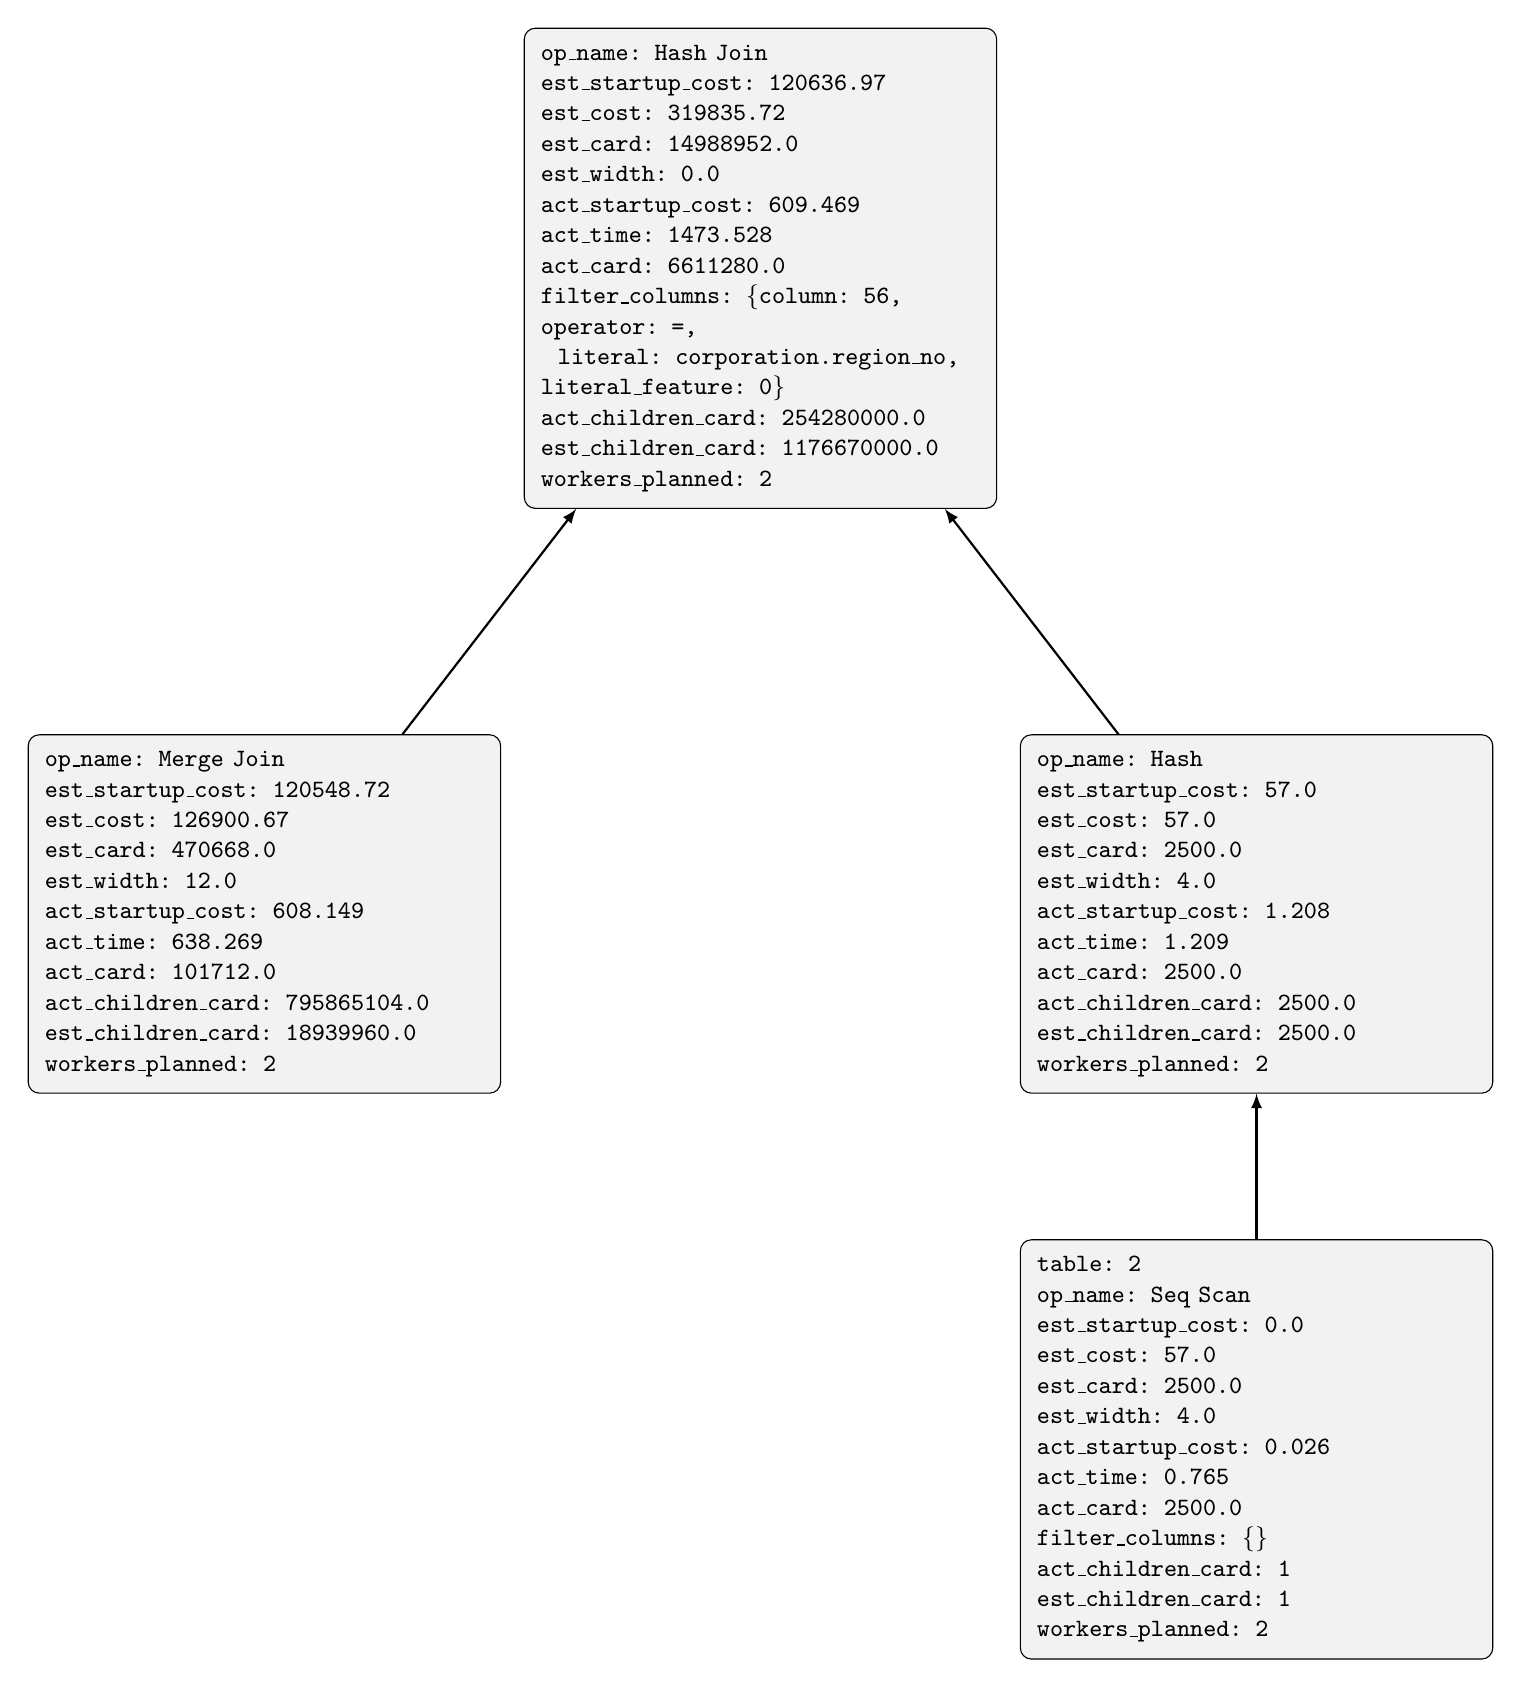
\begin{tikzpicture}[
    planop/.style={draw, rounded corners, fill=gray!10, align=left, inner sep=6pt, text width=0.46\linewidth, font=\small}
  ]
    \node[planop] (join) at (0,0) {%
      \texttt{op\_name: Hash Join}\\
      \texttt{est\_startup\_cost: 120636.97}\\
      \texttt{est\_cost: 319835.72}\\
      \texttt{est\_card: 14988952.0}\\
      \texttt{est\_width: 0.0}\\
      \texttt{act\_startup\_cost: 609.469}\\
      \texttt{act\_time: 1473.528}\\
      \texttt{act\_card: 6611280.0}\\
      \texttt{filter\_columns: \{column: 56, operator: =,}\\
      \texttt{\ \ literal: corporation.region\_no,\ literal\_feature: 0\}}\\
      \texttt{act\_children\_card: 254280000.0}\\
      \texttt{est\_children\_card: 1176670000.0}\\
      \texttt{workers\_planned: 2}
    };
    \node[planop] (left) at (-6.3,-8.2) {%
      \texttt{op\_name: Merge Join}\\
      \texttt{est\_startup\_cost: 120548.72}\\
      \texttt{est\_cost: 126900.67}\\
      \texttt{est\_card: 470668.0}\\
      \texttt{est\_width: 12.0}\\
      \texttt{act\_startup\_cost: 608.149}\\
      \texttt{act\_time: 638.269}\\
      \texttt{act\_card: 101712.0}\\
      \texttt{act\_children\_card: 795865104.0}\\
      \texttt{est\_children\_card: 18939960.0}\\
      \texttt{workers\_planned: 2}
    };
    \node[planop] (hash) at (6.3,-8.2) {%
      \texttt{op\_name: Hash}\\
      \texttt{est\_startup\_cost: 57.0}\\
      \texttt{est\_cost: 57.0}\\
      \texttt{est\_card: 2500.0}\\
      \texttt{est\_width: 4.0}\\
      \texttt{act\_startup\_cost: 1.208}\\
      \texttt{act\_time: 1.209}\\
      \texttt{act\_card: 2500.0}\\
      \texttt{act\_children\_card: 2500.0}\\
      \texttt{est\_children\_card: 2500.0}\\
      \texttt{workers\_planned: 2}
    };
    \node[planop] (scan) at (6.3,-15.0) {%
      \texttt{table: 2}\\
      \texttt{op\_name: Seq Scan}\\
      \texttt{est\_startup\_cost: 0.0}\\
      \texttt{est\_cost: 57.0}\\
      \texttt{est\_card: 2500.0}\\
      \texttt{est\_width: 4.0}\\
      \texttt{act\_startup\_cost: 0.026}\\
      \texttt{act\_time: 0.765}\\
      \texttt{act\_card: 2500.0}\\
      \texttt{filter\_columns: \{\}}\\
      \texttt{act\_children\_card: 1}\\
      \texttt{est\_children\_card: 1}\\
      \texttt{workers\_planned: 2}
    };

    \draw[-latex, thick] (left) -- (join);
    \draw[-latex, thick] (hash) -- (join);
    \draw[-latex, thick] (scan) -- (hash);
  \end{tikzpicture}
  }
  \caption[Top-node Cutout with Hash Join from ZeroShot Data]{Top-node tree cutout of one \texttt{parsed\_plan} with a \texttt{Hash Join} from \path{credit/workload_100k_s1_c8220}. Child relationships are shown by arrows,
   and each node box contains selected \texttt{plan\_parameters} of that node for the displayed cutout.}
  \label{fig:parsed-plan-hash-join-cutout}
\end{figure}

Figure~\ref{fig:parsed-plan-hash-join-cutout} shows such a structured plan representation for a \texttt{Hash Join} and its children, directly taken from the ZeroShot benchmark data~\parencite{zeroshot}.
Here, data like cardinalities and filter predicates can be retrieved from the \texttt{filter\_columns} field.
Furthermore, PostgreSQL-specific fields like \texttt{workers\_planned} (planned parallel workers for the node) are available.

In \texttt{zeroshot\_to\_t3.py}, we convert this tree recursively into the same nested operator structure
that the original T3 implementation expects
for Umbra plans~\parencite{t3}.
The PostgreSQL-specific temporary operators \texttt{hash} and \texttt{materialize} are mapped to the abstract operator \texttt{temp}.
Consequently, every converted node additionally stores a copy of the original \texttt{plan\_parameters} under a dedicated \texttt{pg} payload.
Training and inference, that use PostgreSQL-native features, read from this payload and from the pipeline layout.

T3 also requires database schema information. However, the Zero-Shot data does not provide this information, so a minimal placeholder schema is used instead.

The pipeline assignment is stored in the \texttt{analyzePlanPipelines} list of the converted plan.
For every pipeline, we also derive start and stop times from the per-node actual timings in \texttt{plan\_parameters}.
These pipeline durations are not used by the primary model,
but are available for the per-pipeline and per-tuple prediction variants evaluated in the ablation study
(Section~\ref{sec:evaluation_ablation}).


\section{Feature Vector Construction}

As PostgreSQL plans contain different data, we use \texttt{pg\_features.py} to construct the feature vector for each pipeline after the pipeline decomposition.
Subsequently, the \texttt{plan\_parameters} are kept in the converted tree (\texttt{pg} payload entry), as we use them for the feature extraction.

Each pipeline's feature vector consists of two concatenated blocks, as Figure~\ref{fig:pg-feature-vector-snippet} shows:

\begin{enumerate}
  \item \textbf{Pipeline-level aggregates.}
  From the available \texttt{pg} payload, we extract as much distinct information as possible.

  Therefore, we start by summarizing different information categories per pipeline with sum, max, and average statistics.
  First, the \texttt{pg\_card\_...} fields capture output cardinality summaries.

  Insights about PostgreSQL-specific cost, parallelism, and width features are captured in the
  \texttt{pg\_est\_cost\_...},
  \texttt{pg\_est\_startup\_...},
  \texttt{pg\_workers\_planned\_sum}
  and \texttt{pg\_est\_width\_avg} fields.

  Further, the \texttt{pg\_num\_(scan/join/sort/etc.)} family counts operator classes.

  Moreover, the \texttt{pg\_scan\_has\_filter}
  and \texttt{pg\_filter\_(and/or/compare/like/in)} counters enumerate scan predicate attributes.

  Finally, pipeline-context features describe structure using
  \texttt{pg\_pipeline\_num\_ops} for instance.
  \item \textbf{Operator-level block.}
  For every operator that occurs in \texttt{parsed\_plans}, we assign a slice in the feature vector.
  If multiple operators of the same type occur in the pipeline, we sum the features over all occurences.
  In Figure~\ref{fig:pg-feature-vector-snippet}, the excerpt of the operator-type block for the \texttt{Nested\_Loop join} operator is depicted.

  Depending on the operator type, we include different features. This feature set is derived from T3's Umbra implementation~\parencite{t3}.
  For example, a join would include different features than a scan, like in the Umbra/T3 approach.

  Regarding the calculations of the features, we follow the Umbra/T3 implementation where adequate.
  A deviation would be, e.\,g., how expression percentages are formed due to the different nature of PostgreSQL's filter predicates (CITE).

  Finally, we include the operator count ``\texttt{const}'', which exists for every operator type in both our and the Umbra/T3 implementation~\parencite{t3}.
\end{enumerate}

\begin{figure}[htpb]
  \centering
  \footnotesize
  \setlength{\tabcolsep}{5pt}
  \begin{tabular}{@{}l r@{}}
    \toprule
    \multicolumn{2}{@{}l}{\emph{Pipeline-level block (excerpt; first 12 of 23 features)}} \\
    \midrule
    \texttt{pg\_card\_sum} & 6541.0 \\
    \texttt{pg\_card\_max} & 6537.0 \\
    \texttt{pg\_est\_cost\_sum} & 16882.95 \\
    \texttt{pg\_est\_cost\_max} & 16877.3 \\
    \texttt{pg\_est\_startup\_sum} & 125.82 \\
    \texttt{pg\_workers\_planned\_sum} & 4.0 \\
    \texttt{pg\_est\_width\_avg} & 10.0 \\
    \texttt{pg\_num\_scan} & 1.0 \\
    \texttt{pg\_num\_join} & 1.0 \\
    \texttt{pg\_scan\_has\_filter} & 0.0 \\
    \texttt{pg\_filter\_compare\_count} & 0.0 \\
    \texttt{pg\_pipeline\_num\_ops} & 2.0 \\
    \midrule
    \multicolumn{2}{@{}l}{\emph{Operator-type block (excerpt; Nested\_Loop slice; 130 entries in full)}} \\
    \midrule
    \texttt{Nested\_Loop\_const} & 1.0 \\
    \texttt{Nested\_Loop\_in\_percentage} & 0.11473152822395594 \\
    \texttt{Nested\_Loop\_right\_card} & 98378.0 \\
    \texttt{Nested\_Loop\_out\_percentage} & 0.008260670032124828 \\
    \multicolumn{2}{@{}c@{}}{\scriptsize\textit{(remaining operator-type entries omitted)}} \\
    \bottomrule
  \end{tabular}
  \caption[Excerpt of a PostgreSQL-native Pipeline Feature Vector]
  {Excerpts of the pipeline-level block (first twelve features) and of the \texttt{Nested\_Loop} operator entries in the operator-type block.
  They are from one pipeline of query \texttt{index\_workload\_100k\_s2\_c8220\_890} on the TPC-H database.
  The full vector has 153 dimensions; remaining pipeline and operator entries are omitted.}
  \label{fig:pg-feature-vector-snippet}
\end{figure}

